% =========================================================================
% CAPITOLO 6 — IL SUBSTRATO DI MACHINE LEARNING
% =========================================================================

\chapter{Il substrato di machine learning}
\label{ch:data_pipeline}

\noindent
{\rmfamily\itshape
\begin{tabular}[t]{@{}l@{\hspace{0.3cm}}p{12.5cm}@{}}
\textls[50]{\textbf{Trattati:}} &
\textls[50]{Struttura latente · Riduzione della dimensionalità · Geometria della varietà · Segnali di preallarme
· Pseudo-replicazione e risultati nulli · Rilevamento di anomalie · Osservazione vs rianalisi}
\end{tabular}
}

\vspace{0.5cm}

Questo capitolo è il cuore della fase di \emph{rilevamento}: l'analisi che recupera, dal record osservativo dell'AMOC, la struttura latente che la fase di \emph{traduzione} renderà poi percepibile. Realizza gli obiettivi O1.1--O1.3 e testa le ipotesi analitiche H1--H3. Lo scopo non è una nuova affermazione sull'oceano --- chi cerca una scoperta oceanografica non ne troverà una qui, ed è voluto. È più ristretto e, per questa tesi, più importante: stabilire con evidenza che la struttura verticale dell'AMOC si riduce a un piccolo insieme di coordinate fedeli e interpretabili, perché tutto ciò che la rappresentazione fa nel Capitolo~\ref{ch:translate} poggia sull'affidabilità di quel substrato. I risultati sono quindi inquadrati dalle loro implicazioni per la rappresentazione anziché dal loro significato oceanografico. L'analisi usa l'analisi delle componenti principali --- la classica decomposizione lineare del campo, equivalente alle funzioni ortogonali empiriche standard nella scienza del clima --- e poi la verifica rispetto a un autoencoder non lineare, che funge da controllo su se un metodo più flessibile recuperi qualche struttura che le coordinate lineari non colgono.

Il materiale è il record RAPID-MOCHA-WBTS a \ang{26.5}~nord: la funzione di corrente del rovesciamento campionata su 307 livelli di profondità nel periodo da aprile 2004 a marzo 2024. I record incompleti verso la fine della serie sono scartati, il che lascia 14{,}596 profili, ciascuno un vettore di 307 numeri che descrive come il trasporto è distribuito con la profondità.\footnote{La griglia di profondità è quasi uniforme (spaziatura 19,33--19,87~m, mediana 19,59~m; rapporto max/min di 1,03), perciò non si applica alcuna ponderazione per lo spessore degli strati: con livelli così uniformemente spaziati, la ponderazione scalerebbe ogni livello di una costante quasi identica, che la PCA assorbe senza alcun effetto sui loading o sulle quote di varianza.} Prima di tutto, ogni profilo è centrato sulla media del record, così che l'analisi descriva come la struttura verticale \emph{si discosta} dalla sua forma media anziché recuperare semplicemente di nuovo quella forma media. I profili non sono deliberatamente destagionalizzati: lo scopo è rappresentare gli stati che l'oceano ha effettivamente occupato, perciò il ciclo annuale è mantenuto come parte della variabilità reale che l'osservatore vede anziché filtrato via. Il costo, detto chiaramente, è che la ricorrenza che la Scena~II fa poi emergere è in parte stagionale.

% -------------------------------------------------------------------------
\section{Struttura latente e decomposizione PCA}
\label{sec:detect-pca}

Il primo obiettivo (O1.1) trova i modi dominanti della variabilità verticale dell'AMOC tramite analisi delle componenti principali, e il risultato è netto: la variabilità è quasi unidimensionale. Un singolo modo spiega l'\SI{89.82}{\percent} della varianza e due insieme il \SI{97.86}{\percent} (Tabella~\ref{tab:pca-variance}); dal terzo modo in poi ciascuno aggiunge meno dell'\SI{1.6}{\percent}, e la curva scree si piega nettamente tra il secondo e il terzo --- il familiare gomito dove la struttura finisce e inizia il rumore. Questo conferma H1 con ampio margine: l'ipotesi si aspettava due o tre modi sopra l'\SI{80}{\percent} (\S\ref{sec:hypotheses}), e i dati ne danno due sopra il \SI{97}{\percent}.

% it/figures/data_pipeline/tab_pca_variance.tex — versione italiana
\begin{table}[!ht]
    \centering
    \small
    \caption[Varianza spiegata dai modi PCA verticali.]{Varianza spiegata
    da ciascuna componente principale dei profili verticali dell'AMOC. Due modi
    raggiungono il \SI{97.86}{\percent}; la coda oltre la PC2 è rumore.}
    \label{tab:pca-variance}
    \begin{tabular}{@{}lrr@{}}
        \toprule
        \textbf{Modo} & \textbf{Varianza} & \textbf{Cumulata} \\
        \midrule
        PC1 & 89.82\% & 89.82\% \\
        PC2 &  8.03\% & 97.86\% \\
        PC3 &  1.57\% & 99.42\% \\
        PC4 &  0.37\% & 99.80\% \\
        PC5 &  0.12\% & 99.91\% \\
        PC6 &  0.05\% & 99.97\% \\
        \bottomrule
    \end{tabular}
\end{table}

% it/figures/data_pipeline/fig_pca_scree.tex — versione italiana
\begin{figure}[!ht]
    \centering
    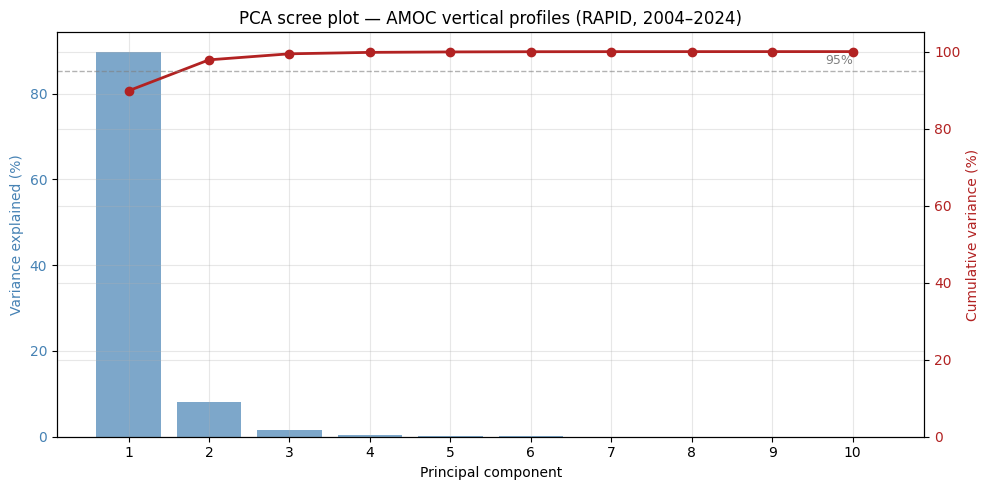
\includegraphics[width=0.8\textwidth]{figures/data_pipeline/pca_scree.png}
    \caption[Varianza spiegata dai modi PCA verticali.]{\textbf{La variabilità
    verticale dell'AMOC è quasi monodimensionale.} Varianza spiegata da ciascuna
    componente principale dei profili verticali a 307 livelli. Il primo modo da solo
    spiega il \SI{89.82}{\percent} e i primi due insieme il \SI{97.86}{\percent};
    il netto gomito dopo il secondo modo segna dove la struttura cede al rumore.
    Questo è lo spazio latente a due coordinate su cui è costruita la rappresentazione
    esperienziale.}
    \label{fig:pca-scree}
\end{figure}


Entrambi i modi hanno un chiaro significato fisico. PC1 ha lo stesso segno a ogni profondità e culmina intorno ai 1150~m, vicino a dove culmina il profilo medio (\S\ref{subsec:scene-column}): quando sale l'intera cella di rovesciamento si rafforza mantenendo la sua forma, quando scende la cella si indebolisce nel suo insieme. PC1 è l'\emph{intensità} della circolazione --- vicino al novanta per cento di ciò che l'AMOC fa da un giorno all'altro. PC2 cambia segno una volta scendendo lungo la colonna d'acqua, rafforzando la cella a una profondità mentre la indebolisce a un'altra: la \emph{ridistribuzione verticale} della circolazione, uno spostamento minore ma genuino della sua forma attorno alla media.

% it/figures/data_pipeline/mode_shapes.tex — versione italiana
\begin{figure}[!ht]
    \centering
    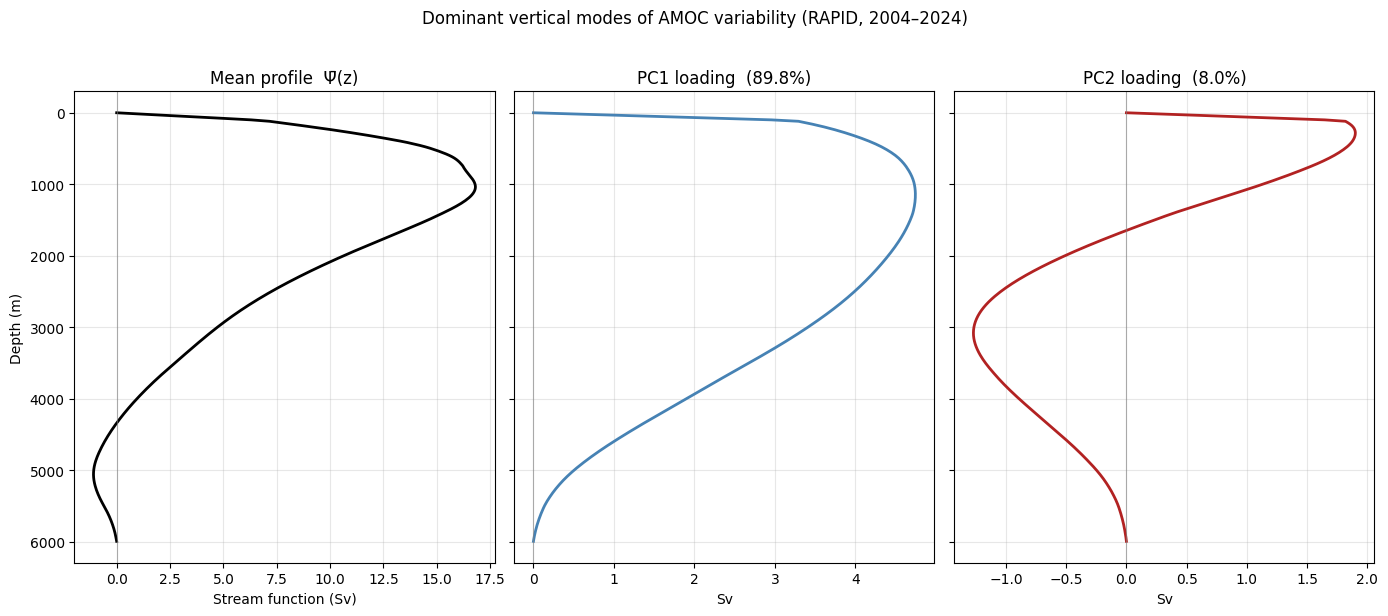
\includegraphics[width=1\textwidth]{figures/data_pipeline/mode_shapes.png}
    \caption[I due modi verticali: intensità e ridistribuzione.]{\textbf{I due
    modi che spiegano l'anatomia verticale dell'AMOC.} Ogni curva è un profilo di
    loading tracciato rispetto alla profondità. La PC1 (intensità) è un \emph{monopolo}:
    lo stesso segno a ogni profondità, con picco attorno a 1150~m, vicino alla profondità
    a cui il profilo medio ha il suo picco, così che un cambiamento nel suo score rafforza
    o indebolisce coerentemente l'intera cella di rovesciamento.
    La PC2 (ridistribuzione) è un \emph{dipolo}: cambia segno una volta con la profondità,
    rafforzando la cella a un livello mentre la indebolisce a un altro. I loading sono
    scalati in Sv per la visualizzazione. Insieme queste due forme portano il
    \SI{97.86}{\percent} della variabilità verticale.}
    \label{fig:mode-shapes}
\end{figure}


È qui che l'analisi tocca per la prima volta direttamente la tesi. Sarebbe facile assegnare significati a questi modi a posteriori; non è ciò che accade qui. Il modo di intensità è recuperato dai dati e poi confermato rispetto a un evento noto, che è una posizione più solida da cui argomentare. Seguito nel tempo, PC1 cala bruscamente durante il 2009--2010 --- l'indebolimento più accuratamente documentato del record osservativo --- raggiungendo un punteggio medio di periodo di PC1 di $-23.97$ rispetto a una media sull'intero record pari a zero.\footnote{Lo stesso evento del 2009--2010 compare indipendentemente nel campo grezzo profondità--tempo, in questa serie di intensità, e più avanti nel rilevatore di anomalie: tre metodi, un episodio fisico.} Che una singola linea possa ancora portare un evento visto per la prima volta nell'intero campo profondità--tempo è una prova piccola ma reale dell'affermazione della tesi --- che questo sistema può essere ri-rappresentato in meno dimensioni senza perdere ciò che conta. Il piano PC1--PC2, che tiene il \SI{97.86}{\percent} dell'anatomia verticale in sole due coordinate, è lo spazio latente lungo cui i profili respireranno fedelmente nel tempo nella condizione esperienziale del Capitolo~\ref{ch:translate}.

% -------------------------------------------------------------------------
\section{Una geometria della varietà essenzialmente piatta}
\label{sec:detect-ae}

Poiché la PCA è un metodo lineare, una domanda importante è se una rappresentazione lineare sia sufficiente a catturare la struttura dei dati dell'AMOC: se la geometria sottostante fosse fortemente non lineare, una proiezione lineare potrebbe semplificarla eccessivamente e perdere informazione. Il confronto che segue è interpretabile grazie a un risultato noto: un autoencoder con attivazioni lineari recupera lo stesso sottospazio della PCA, perciò qualsiasi vantaggio che un autoencoder non lineare mostri a dimensionalità pari è attribuibile alla curvatura della varietà dei dati \citep{baldi1989}. Uno scarto quasi nullo è quindi evidenza di piattezza, non meramente di un pareggio. Il secondo obiettivo (O1.2) testa quindi questa assunzione confrontando la PCA con un autoencoder non lineare addestrato sugli stessi 14{,}596 profili AMOC. Entrambi i modelli sono valutati usando lo stesso numero di dimensioni latenti. Se la struttura latente fosse genuinamente non lineare, ci si aspetterebbe che l'autoencoder ricostruisca i dati più accuratamente. In caso contrario, la PCA dovrebbe comportarsi altrettanto bene.

I risultati sostengono chiaramente la seconda ipotesi. Attraverso le dimensioni latenti da una a cinque l'autoencoder non lineare non ha mai superato la PCA, che è stata costantemente migliore di $-0.06$ a $-0.15$ punti percentuali (Tabella~\ref{tab:ae-gap}); alle due dimensioni usate ovunque, la PCA ha ricostruito il \SI{97.86}{\percent} contro il \SI{97.77}{\percent} dell'autoencoder.\footnote{I livelli di superficie e di fondale sono stati esclusi dall'input dell'autoencoder perché la funzione di corrente è fissata a zero a entrambi i confini per conservazione della massa e quindi non contiene varianza apprendibile.} Questo conferma H2: pur libero di apprendere trasformazioni non lineari, l'autoencoder non ha trovato alcuna struttura significativa oltre la rappresentazione lineare PCA.

% it/figures/data_pipeline/tab_ae_gap.tex — versione italiana
\begin{table}[!ht]
    \centering
    \small
    \caption[Autoencoder contro PCA a dimensione latente appaiata.]{Ricostruzione
    dei profili verticali da parte di un autoencoder non lineare contro la PCA lineare,
    a dimensione latente $k$ appaiata. Lo scarto è negativo a ogni $k$: la PCA non è mai
    battuta, quindi la varietà è piatta. Gli scarti sono calcolati da valori non
    arrotondati, perciò possono differire di 0.01 dalla differenza delle colonne
    arrotondate.}
    \label{tab:ae-gap}
    \begin{tabular}{@{}crrr@{}}
        \toprule
        \textbf{$k$} & \textbf{PCA cum.\ \%} & \textbf{AE $R^2_{\mathrm{Sv}}$ \%} & \textbf{Scarto (pp)} \\
        \midrule
        1 & 89.82 & 89.67 & $-0.15$ \\
        2 & 97.86 & 97.77 & $-0.08$ \\
        3 & 99.42 & 99.36 & $-0.06$ \\
        4 & 99.80 & 99.74 & $-0.06$ \\
        5 & 99.91 & 99.83 & $-0.08$ \\
        \bottomrule
    \end{tabular}
\end{table}

% it/figures/data_pipeline/fig_manifold.tex — versione italiana
\begin{figure}[!ht]
    \centering
    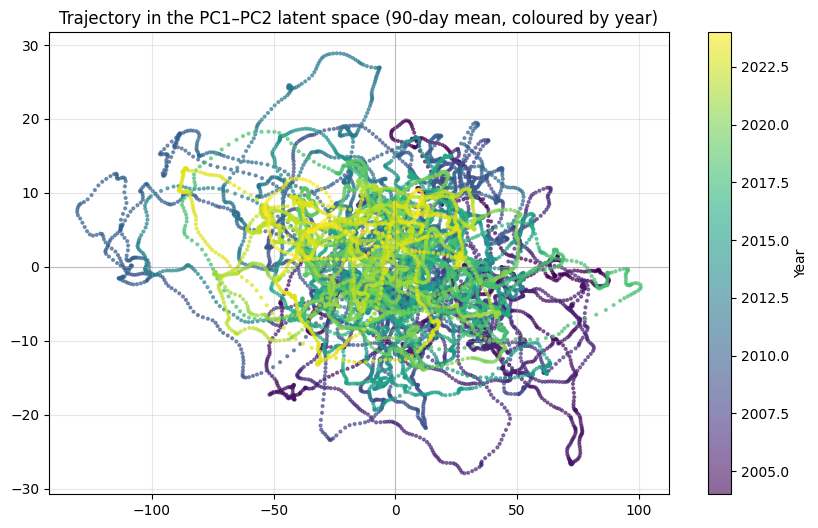
\includegraphics[width=0.85\textwidth]{figures/data_pipeline/fig_manifold.png}
    \caption[La varietà latente piatta dei profili AMOC.]{\textbf{La varietà dei
    profili verticali dell'AMOC è piatta.} Ogni punto è un profilo, collocato dalle
    sue due coordinate latenti --- PC1 (intensità) e PC2 (ridistribuzione verticale).
    Un autoencoder non lineare addestrato sugli stessi profili non li ricostruisce
    meglio della PCA lineare a nessuna dimensione latente (scarto da $-0.06$ a $-0.15$
    punti percentuali; vedi Tabella~\ref{tab:ae-gap}), confermando che due coordinate
    rettilinee catturano la struttura senza distorsione.}
    \label{fig:manifold}
\end{figure}


Questo risultato è importante perché giustifica l'uso delle coordinate latenti lungo l'intera fase di \emph{Traduzione} della tesi. Se la varietà sottostante fosse stata fortemente curva, rappresentare il sistema usando le prime due componenti principali avrebbe introdotto distorsioni forzando una struttura non lineare in uno spazio lineare. Invece, i risultati mostrano che la varietà latente è effettivamente lineare. Di conseguenza, le prime due componenti principali forniscono una rappresentazione tanto altamente interpretabile quanto altamente fedele ai dati originali. Le coordinate possono quindi essere interpretate in modo significativo come modi distinti di variabilità dell'AMOC senza sacrificare l'accuratezza di rappresentazione. In questo caso, l'interpretabilità arriva praticamente a costo nullo in fedeltà, rendendo la rappresentazione proposta tanto scientificamente difendibile quanto adatta come base per le visualizzazioni esperienziali sviluppate nel capitolo seguente.

% -------------------------------------------------------------------------
\section{Segnali di preallarme e risultato nullo}
\label{sec:detect-ews}

Il terzo obiettivo (O1.3) chiede se il record contenga segnali di preallarme di un punto di tipping in avvicinamento. Per la teoria del rallentamento critico, un sistema che si avvicina a una biforcazione mostra varianza crescente e autocorrelazione a lag-1 \citep{dakos2012, scheffer2009}. Testare ciò richiede particolare cura, e qui l'analisi mette in luce un importante problema metodologico.

A prima vista i risultati appaiono molto forti. La varianza mobile della serie di intensità tende al rialzo, con $\tau$ di Kendall $= +0.078$ e un p-value di $2\times10^{-42}$; anche l'autocorrelazione mobile aumenta, con $\tau = +0.088$ e un p-value di $1\times10^{-52}$. Presi alla lettera sarebbero un segnale estremamente forte. L'interpretazione è fuorviante, perché le finestre mobili si sovrappongono sostanzialmente e le migliaia di valori calcolati non sono osservazioni indipendenti.\footnote{Il test di Kendall assume indipendenza. Qui le statistiche mobili usano finestre di 730 profili (un anno) fortemente sovrapposte, perciò i valori consecutivi sono altamente dipendenti --- effetto amplificato dalla forte autocorrelazione della serie originale ($0.943$). Il software restituisce un p-value molto piccolo senza tenere conto di quella dipendenza, facendo apparire il risultato più certo di quanto sia.} Quando si usa invece il numero effettivo di osservazioni indipendenti --- circa 19,5 finestre non sovrapposte di 730 profili --- e il test è corretto di conseguenza, le tendenze apparenti scompaiono. Il p-value corretto per la tendenza della varianza è \textbf{0.634}, mentre per la tendenza dell'autocorrelazione è \textbf{0.595}. Nessuno dei due risultati è statisticamente significativo (Tabella~\ref{tab:ews}). Il forte segnale iniziale era quindi causato dal trattare osservazioni dipendenti come se fossero indipendenti.

% it/figures/data_pipeline/tab_ews.tex — versione italiana
\begin{table}[!ht]
    \centering
    \small
    \caption[Trend di preallarme: significatività ingenua contro corretta.]{Test di
    trend con il $\tau$ di Kendall per i due segnali classici di preallarme. I p-value
    ingenui trattano le finestre sovrapposte come indipendenti; i p-value corretti
    contano le $\sim$19.5 finestre indipendenti che il record contiene. Nessuno dei due
    trend è significativo.}
    \label{tab:ews}
    \begin{tabular}{@{}lcccc@{}}
        \toprule
        \textbf{Segnale} & \textbf{Kendall $\tau$} & \textbf{p ingenuo} & \textbf{p corretto} & \textbf{Verdetto} \\
        \midrule
        Varianza mobile & $+0.078$ & $2\times10^{-42}$ & 0.634 & non significativo \\
        AR(1) mobile     & $+0.088$ & $1\times10^{-52}$ & 0.595 & non significativo \\
        \bottomrule
    \end{tabular}
\end{table}

% it/figures/data_pipeline/fig_ews.tex — versione italiana
\begin{figure}[!ht]
    \centering
    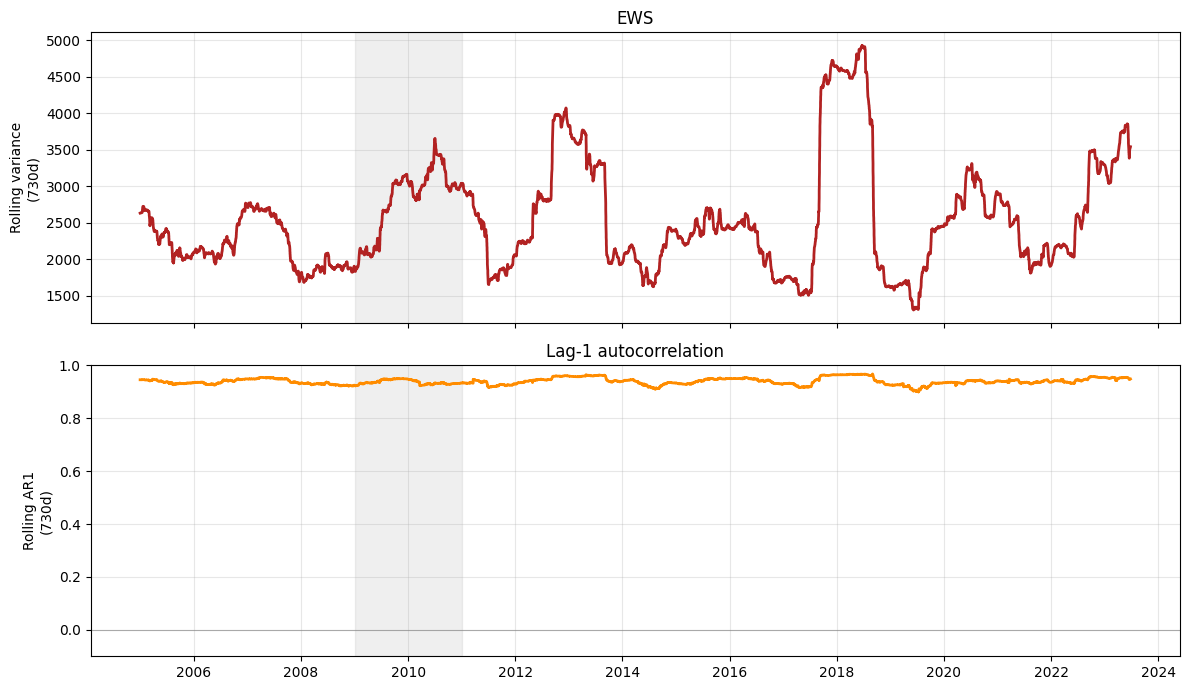
\includegraphics[width=0.9\textwidth]{figures/data_pipeline/ews.png}
    \caption[Segnali di preallarme: varianza mobile e autocorrelazione.]{\textbf{Nessun
    trend di preallarme rigoroso.} Varianza mobile e autocorrelazione a lag~1 della serie
    di intensità lungo il record. Entrambe oscillano senza una salita sostenuta.
    I loro p-value di trend ingenui ($\sim$$10^{-42}$) sono artefatti di finestre
    fortemente sovrapposte; corretti per le $\sim$19.5 finestre indipendenti che il
    record contiene davvero, i trend non sono significativi (p~$=$~0.634 e
    0.595; Tabella~\ref{tab:ews}).}
    \label{fig:ews}
\end{figure}


La conclusione finale è quindi un \emph{risultato nullo}. Una volta considerata correttamente la struttura di dipendenza dei dati, gli indicatori classici di preallarme non possono essere distinti dal rumore. Questo sostiene H3 nella sua forma nulla e rappresenta un importante contributo metodologico anziché un limite. Un risultato positivo ottenuto interpretando male le statistiche sarebbe stato più attraente, ma non sarebbe stato affidabile. Dimostrare che un segnale apparentemente forte scompare una volta affrontata la dipendenza statistica è il risultato sostanziale qui. Indipendentemente da quella correzione, il record è semplicemente troppo breve per la domanda: vent'anni dell'array RAPID sono assai più brevi della scala temporale da multidecennale a centennale su cui si svilupperebbe un tipping dell'AMOC, perciò l'assenza di una tendenza di preallarme qui dice ciò che questo record può sostenere, non se l'AMOC si stia avvicinando a una soglia. Per le stesse ragioni gli indicatori sono calcolati sulla serie di intensità grezza, senza detrending. Rimuovere prima una tendenza lenta è standard nel lavoro sul rallentamento critico, così che varianza e autocorrelazione riflettano le fluttuazioni anziché la tendenza stessa; qui non si fa perché in vent'anni non c'è alcuna tendenza robusta da rimuovere --- i test corretti sono essi stessi non significativi --- e una finestra di detrending è una scelta arbitraria che può fabbricare o cancellare un segnale apparente. Lasciare grezza la serie mantiene il risultato nullo poggiante sulla sola correzione per la dipendenza, al costo che ogni tendenza residua, e il ciclo stagionale mantenuto, restano nella varianza che gli indicatori misurano. Il confine tra rilevamento di pattern e predizione che questa fase osserva è registrato nell'Appendice~\ref{app:limits-detect}.

% -------------------------------------------------------------------------
\section{Rilevamento di anomalie}
\label{sec:detect-anomalies}

L'analisi di preallarme cerca lente \emph{tendenze}; una domanda diversa riguarda singoli \emph{eventi} --- quali momenti si discostano dal comportamento normale. Un Isolation Forest sulle coordinate PC1--PC2 segnala il \SI{5}{\percent} del record (730 profili) come anomalo, concentrato nel 2009--2010 (158 profili), 2012--2013 (100 profili) e 2018 (66 profili). Il punteggio di anomalia non aumenta nel tempo: i momenti insoliti sono distribuiti lungo il record anziché accumularsi verso la fine, un'altra indicazione che il sistema non si sta muovendo progressivamente verso una soglia.

% it/figures/data_pipeline/fig_anomalies.tex — versione italiana
\begin{figure}[!ht]
    \centering
    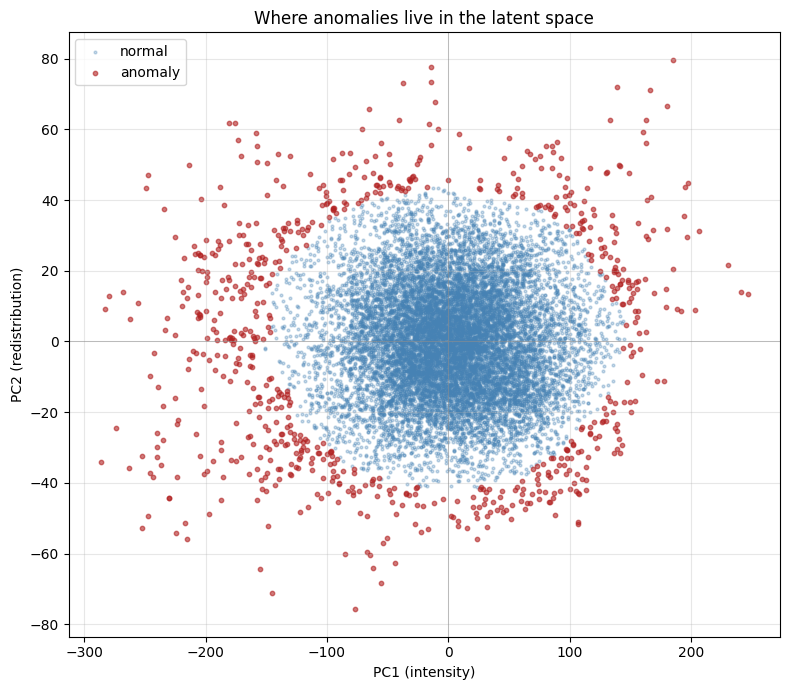
\includegraphics[width=0.9\textwidth]{figures/data_pipeline/anomalies.png}
    \caption[Anomalie Isolation Forest lungo il record.]{\textbf{Eventi anomali
    discreti, distribuiti lungo il record.} L'Isolation Forest segnala il
    \SI{5}{\percent} dei profili (730) come anomali nel piano PC1--PC2. Si addensano
    nel 2009--2010 (158 profili), nel 2012--2013 (100) e nel 2018 (66), senza trend nel
    tempo --- a conferma del risultato nullo di preallarme da un metodo diverso. Questi
    momenti diventano texture percepibile (principio di grammatica~P3) nel
    Capitolo~\ref{ch:translate}.}
    \label{fig:anomalies}
\end{figure}


Due aspetti sono importanti per questa tesi. Primo, questa analisi sostiene il risultato nullo da una prospettiva completamente indipendente: un algoritmo che non si basa sulla teoria del preallarme non trova anch'esso alcuno spostamento graduale, ma piuttosto eventi isolati distribuiti lungo il record ventennale. Raggiunge la stessa conclusione con un metodo diverso.\footnote{I cluster di anomalie corrispondono a caratteristiche identificate indipendentemente --- l'indebolimento del 2009--2010 e i picchi di varianza del 2012--2013 e del 2018 --- con il \SI{41.4}{\percent} dei profili anomali che ricade nel quarto più alto di varianza locale. Metodi diversi rivelano lo stesso comportamento fisico.} Secondo, queste anomalie forniscono la base per una specifica decisione di design. Seguendo la grammatica introdotta nel Capitolo~\ref{ch:literature}, gli scostamenti dal regime normale possono essere tradotti in cambiamenti locali di texture percettiva (principio~P3). I momenti identificati dal rilevatore sono quindi gli stessi momenti che la rappresentazione esperienziale trasformerà in cambiamenti percepibili --- il che significa che il rilevamento di anomalie non è solo un risultato sull'AMOC, ma anche un input diretto per come l'AMOC è rappresentata.

% -------------------------------------------------------------------------
\section{Osservazione a confronto con la rianalisi}
\label{sec:detect-copernicus}

Il passo finale confronta le osservazioni RAPID con l'ensemble di rianalisi Copernicus GREP sui 237 mesi che condividono, per caratterizzare quanto bene la rianalisi riproduca il segnale osservato e per identificare l'incertezza che la fase di \emph{traduzione} deve comunicare. L'accordo è moderato: correlazione 0,754, un piccolo bias di $+0.584$~Sv con RAPID leggermente più forte, e una differenza quadratica media di 2,300~Sv. Entrambi restano vicini ai 17~Sv e variano in modo simile nel tempo, perciò la rianalisi cattura il comportamento complessivo della circolazione anche dove sbaglia singoli mesi.

Il risultato più informativo riguarda la copertura dell'incertezza. RAPID ricade entro l'intervallo di $\pm1$ deviazione standard dell'ensemble di rianalisi solo nel \SI{40.1}{\percent} dei mesi.\footnote{Se la dispersione dell'ensemble rappresentasse una stima ben calibrata della propria incertezza, l'osservazione dovrebbe ricadere entro l'intervallo di una deviazione standard molto più spesso. Una copertura più bassa indica che la dispersione è troppo stretta rispetto agli errori effettivi.} Un ensemble di modelli con un intervallo di incertezza realistico dovrebbe catturare l'osservazione più frequentemente. Questa bassa copertura indica che l'ensemble è \emph{troppo sicuro di sé}: l'incertezza che riporta è minore dell'errore reale. Questo punto è importante per la tesi perché la dispersione dell'ensemble è esattamente ciò che la fase di \emph{traduzione} converte in incertezza percepibile, secondo il principio~P4 della grammatica di design. Comprendere che questa incertezza è sottostimata è quindi parte del rappresentarla onestamente: la visualizzazione può comunicare l'incertezza del modello chiarendo al contempo che l'incertezza reale è probabilmente maggiore.

% -------------------------------------------------------------------------
\section{Sintesi analitica}
\label{sec:detect-summary}

La fase analitica consegna alla fase di \emph{traduzione} un substrato documentato anziché assunto. Due coordinate interpretabili --- intensità e ridistribuzione verticale --- portano il \SI{97.86}{\percent} della variabilità verticale dell'AMOC, e un modello non lineare conferma che la varietà è abbastanza piatta da usarle senza distorsione rilevante. Il record non mostra alcuna tendenza robusta di preallarme ma contiene anomalie discrete che possono diventare texture percettiva, e il confronto con la rianalisi fornisce una stima dell'incertezza fisicamente significativa, benché troppo stretta. Ciascuno è un input giustificato per un substrato compatto, fedele, interpretabile, consapevole degli eventi e portatore di incertezza, su cui un sistema invisibile può essere reso percepibile senza essere travisato.
